\documentclass[11pt,aspectratio=169]{beamer}

\usepackage{rcstalk}
\usetheme{rcstheme}

\topic{File systems}
\subtitle{Lecture 12: File systems}

\usepackage{tikz}
\usetikzlibrary{positioning,shapes,fit,backgrounds,shadows,chains}

\newcommand{\map}[3]{\leavevmode%
\hbox to1in{\Maroon{#1}\rightarrowfill}%
\Blue{\framebox[1in][c]{\strut #2}}%
\hbox to1in{\rightarrowfill\Maroon{#3}}}

\begin{document}

\maketitle

\begin{slide}{File system fun}
\itms{
  \item File systems: traditionally hardest part of OS
  \ittms{
    \item More papers on FSes than any other single topic
  }
  \item Main tasks of file system:
  \ittms{
    \item Don't go away (ever)
    \item Associate bytes with name (files)
    \item Associate names with each other (directories)
      
    \item Can implement file systems on disk, over network, in memory, in non-volatile ram (NVRAM), on tape, w/ paper.
    \item We'll focus on disk and generalize later
  }
  \item Today: files, directories, and a bit of performance
}
\end{slide}

\begin{slide}{Why disks are different}
\itms{
  \item Disk = First state we've seen that doesn't go away\\[-.5ex]
\hspace*{2em}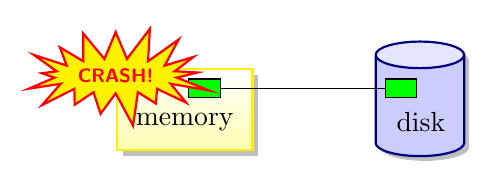
\begin{tikzpicture}
\path (3,0) node (disk) {disk}
   +(120:5mm) node[draw,fill=green,minimum width=4mm] (data) {};
\path (0,0) node (mem) {memory}
   +(60:5mm) node[draw,fill=green,minimum width=4mm] (data2) {};
\begin{scope}[on background layer]
\node[cylinder, shape border rotate=90,shape aspect=0.3,
    fit=(disk) (data), drop shadow={shadow xshift=.4ex,shadow
        yshift=-.4ex}] {};
\node[draw=blue!50!black!100,thick,cylinder,
    shape border rotate=90,shape aspect=0.3,
    fit=(disk) (data),
     cylinder uses custom fill,
     cylinder body fill=blue!20,cylinder end fill=blue!10] {};
\node[top color=white,bottom color=yellow!30,draw=yellow,thick,
    fit=(mem) (data2),drop shadow,name=membox] {};
\end{scope}
\node[outer sep=0pt,starburst,fill=yellow,draw=red,thick,text=red,
    text opacity=1,font=\sffamily\bfseries\scriptsize,inner sep=2pt,
    starburst points=17,random starburst=8,starburst point height=5mm,
    yshift=-1mm]
      at (membox.north west) {CRASH!};
\draw (data) -- (data2);
\end{tikzpicture}
  \ittms{
    \item   So: Where all important state ultimately resides
  }
  \item  Slow (milliseconds access vs.\ nanoseconds for memory)
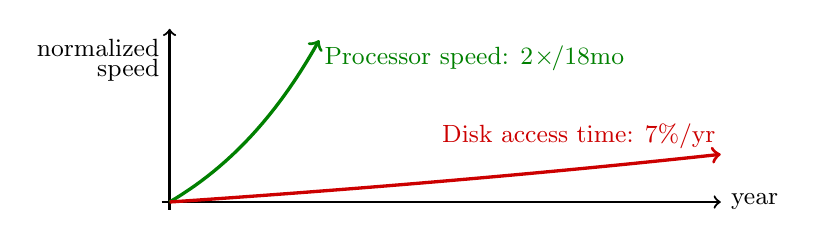
\begin{tikzpicture}[very thick,font=\normalfont\small]
\draw[->,thick] (0mm,-1mm) -- (0mm,2.2cm) node[below left,align=right]
     {normalized\\[-1ex]speed};
\draw[->,thick] (-1mm,0mm) -- (7cm,0mm) node[right] {year};
\draw[color=green!50!black,->] plot[domain=0:1.90]
     (\x,{exp(0.587786664902*\x)-1})
     node[below right=-1mm] {Processor speed: $2\!\times\!\!/18\mathrm{mo}$};
\draw[color=red!80!black,->] plot[domain=0:7]
     (\x,{exp(0.0676586484738*\x)-1})
     node[above left=-1mm] {Disk access time: $7\%/\mathrm{yr}$};
\end{tikzpicture}
\vspace*{-1ex}
  \item Huge (100--1,000x bigger than memory)
  \ittms{
    \item How to organize large collection of ad hoc information?
    \item Taxonomies!   (Basically FS = general way to make these)
  }
}
\end{slide}

% Memory and disk numbers from pricewatch
% 
% Flash numbers based on intel product
% http://www.intel.com/design/flash/nand/extreme/index.htm
\begin{slide}{Disk vs.\ Memory}
\centerline{\begin{tabular}{|l|c|c|c|}
\cline{2-4}
\multicolumn{1}{l|}{} & & MLC NAND & \\
\multicolumn{1}{l|}{} & Disk & Flash & DRAM \\
\hline
Smallest write   & sector  & sector            & byte \\
Atomic write     & sector  & sector            & byte/word \\
Random read      &  8 ms   & 75 $\mu\mathrm s$ & 50 ns \\
Random write     &  8 ms   & 300 $\mu\mathrm s$*& 50 ns \\
Sequential read  &100 MB/s & 250 MB/s          & $>$ 1 GB/s \\
Sequential write &100 MB/s & 170 MB/s*         & $>$ 1 GB/s \\
Cost             & \$0.04/GB& \$0.65/GB         & \$10/GiB \\
Persistence      & Non-volatile & Non-volatile & Volatile \\
\hline
\end{tabular}}

\bigskip
*Flash write performance degrades over time
\end{slide}

%% \begin{slide}{Disk vs.\ Memory}
%% \centerline{
%% \begin{minipage}[t]{2.5in}
%% \itms{
%%   \item Smallest write: sector
%%   \item Atomic write = sector
%%   \item Random access: $\sim 8\>\rm ms$
%%   \ittms{
%%     \item Not on a good curve
%%   }
%%   \item Seq access: $200\>\rm MB/s$
%%   \item Cost: \$.08--1/GB
%%   \item Contents non-volatile
%%   \ittms{
%%     \item Survives after power failure or reboot
%%   }
%% }
%% \end{minipage}\kern-1ex
%% \begin{minipage}[t]{2.5in}
%% \itms{
%%   \item (Usually) bytes
%%   \item Atomic write byte or word
%%   \item  Random access: $50\>\rm ns$
%%   \ittms{
%%     \item Faster all the time
%%   }
%%   \item Seq access $200$--$1000\>\rm MB/s$
%%   \item Cost: \$10--25/GB
%%   \item Volatile
%%   \ittms{
%%     \item Contents gone after reboot
%%   }
%% }
%% \end{minipage}
%% }
%% \end{slide}

%% \begin{slide}{Flash RAM}
%% \vspace*{-.2in}
%% \itms{
%%   \item Non-volatile read/erase/write memory
%%   \item NOR flash allows byte and word access, like DRAM
%%   \item Cheaper NAND flash requires block access like disks
%%   \ittms{
%%     \item SLC flash (single-level cell) stores one bit per cell
%%     \item MLC stores 2--3 bits/cell, less reliable
%%   }
%%   \item Issues for file systems:
%%   \ittms{
%%     \item No-seek or rotational delays.
%%     \item Currently large transfer delays.
%%     \item Durability issues (limited number of writes per block,
%%       though hidden by drive controller on higher-end devices)
%%   }
%%   \item $\sim$\$6/GB for SLC NAND drive
%%     % (E.g., 80~GB intel SSD selling for \$447)      
%%   \item Some high-end disks now use flash for write caching
%% }
%% \end{slide}



\begin{slide}{Disk review}
\itms{
  \item Disk reads/writes in terms of sectors, not bytes
  \ittms{
    \item Read/write single sector or adjacent groups \\
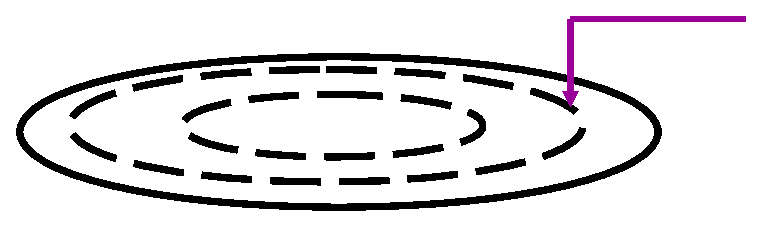
\includegraphics[width=2in]{figs/platter}
  }
  \item How to write a single byte?  ``Read-modify-write''
\vadjust{\moveright 2.75in\vtop to0pt{\hbox{}%
    \rlap{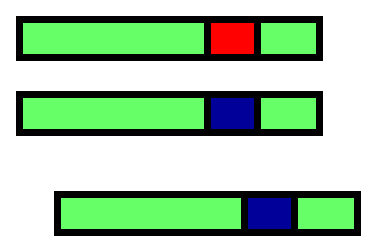
\includegraphics[width=1.75in]{figs/readmodwrite}} \vss}}
  \ittms{
\hsize=4in
    \item Read in sector containing the byte
    \item Modify that byte
    \item Write entire sector back to disk
    \item Key: if cached, don't need to read in
  }
  \item Sector = unit of atomicity. 
  \ittms{
    \item Sector write done completely, even if crash in middle  \\
      (disk saves up enough momentum to complete)
  }
  \item Larger atomic units have to be synthesized by OS
}
\end{slide}

\begin{slide}{Some useful trends}
\itms{
  \item Disk bandwidth and cost/bit improving exponentially
  \ittms{
    \item Similar to CPU speed, memory size, etc.
  }
  \item Seek time and rotational delay improving \emph{very} slowly
  \ittms{
    \item Why? require moving physical object (disk arm)
  }
  \item Disk accesses a huge system bottleneck \& getting worse
  \ittms{
    \item Bandwidth increase lets system (pre-)fetch large chunks for
      about the same cost as small chunk.
    \item Trade bandwidth for latency if you can get lots of
      related stuff. \\
    \item How to get related stuff? Cluster together on disk
  }
  \item Desktop memory size increasing faster than typical workloads
  \ittms{
    \item More and more of workload fits in file cache
    \item Disk traffic changes: mostly writes and new data
    \item Doesn't necessarily apply to big server-side jobs
  }
}
\end{slide}

%% \begin{slide}{The equation that ruled the world}
%% \itms{
%%   \item Approximate time to get data:
%% \Red{$\rm seek\ time(ms) + rotational\ delay(ms)
%%   + bytes/disk\hyph bw$}
%%   \item So?
%%   \ittms{
%%     \item Each time you touch disk = $\sim$10 msec 
%%     \item Touch 100 times = 1 \emph{second}
%%     \item Can do \emph{billions} of ALU ops in same time.
%%   }
%%   \item This fact = Huge social impact on OS research
%%   \ittms{
%%     \item Most pre-2000 research based on speed
%%     \item Publishable speedup = $\sim 30\%$
%%     \item Easy to get $>30\%$ by removing just a few accesses
%%     \item Result: more papers on FSes than any other single topic
%%   }
%% }
%% \end{slide}

\begin{slide}{Files: named bytes on disk}
\itms{
  \item File abstraction:
  \ittms{
    \item User's view: named sequence of bytes \\
      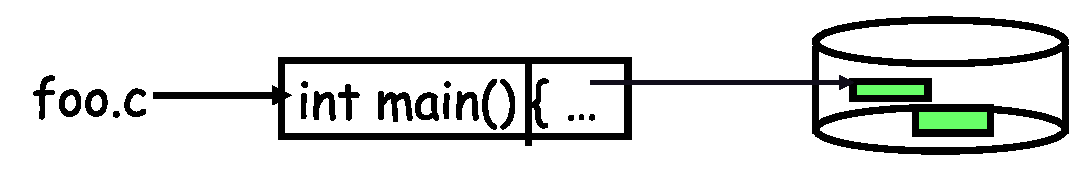
\includegraphics[width=3in]{figs/namedbytes}
\begin{tikzpicture}
\end{tikzpicture}
    \item FS's view: collection of disk blocks
    \item File system's job: translate name \& offset to disk blocks:
	\map{\{file, offset\}}{FS}{disk address}\medskip
  }
  \item File operations:
  \ittms{
    \item Create a file, delete a file
    \item Read from file, write to file
  }
  \item Want: operations to have as few disk accesses as possible \&
    have minimal space overhead (group related things)
}
\end{slide}

\begin{slide}{What's hard about grouping blocks?}
\itms{
%  \item In some sense, the problems we will look at are no different
%    from those in virtual memory
  \item Like page tables, file system metadata are simply data
    structures used to construct mappings\medskip
  \ittms{

    \item Page table: map virtual page \# to physical page \#
    \map{23}{Page table}{33}\medskip

    \item File metadata: map byte offset to disk block address
    \map{512}{Unix inode}{8003121}\medskip

    \item Directory: map name to disk address or file \#
    \map{foo.c}{directory}{44}
  }
}
\end{slide}

\begin{slide}{FS vs.\ VM}
\itms{
  \item In both settings, want location transparency
  %\item Access that can be oblivious to size, \& protection
  \item In some ways, FS has easier job than than VM:
  \ittms{
    \item CPU time to do FS mappings not a big deal (= no TLB)
    \item Page tables deal with sparse address spaces and random access,
      files often denser $(\rm 0 \ldots filesize-1)$, $\sim$sequentially
      accessed
  }
  \item In some ways FS's problem is harder:
  \ittms{
    \item Each layer of translation = potential disk access
    \item Space a huge premium!  (But disk is huge?!?!)  Reason? \\
      Cache space never enough; amount of data you can get in
      one fetch never enough
    \item Range very extreme: Many files $<$10 KB, some files many GB
    %\item Implications?
  }
}
\end{slide}

\begin{slide}{Some working intuitions}
\itms{
  \item FS performance dominated by \# of disk accesses
  \ittms{
    \item Say each access costs $\sim$10 milliseconds
    \item Touch the disk 100 extra times = 1 \emph{second}
    \item Can do a \emph{billion} ALU ops in same time!
  }
  \item Access cost dominated by movement, not transfer:
    \fbox{$\rm \mbox{{\bf \strut seek\ time}}
      + {\bf rotational\ delay}
      + \mbox{\scriptsize\mdseries \# bytes/disk-bw}$}\smallskip
  \ittms{
    \item 1 sector: 5ms + 4ms + 5$\mu$s
      $\left(\mathrm{\approx 512\>B/(100\>MB/s)}\right)$ $\approx$ 9ms
    \item 50 sectors: 5ms + 4ms + .25ms = 9.25ms
    \item Can get \Red{50x the data for only $\sim$3\% more overhead}!
  }
  \item Observations that might be helpful:
  \ittms{
    \item All blocks in file tend to be used together, sequentially
    \item All files in a directory tend to be used together
    \item All names in a directory tend to be used together
    %\item How to exploit?
  }
}
\end{slide}

\begin{slide}{Common addressing patterns}
\itms{
  \item Sequential:
  \ittms{
    \item File data processed in sequential order
    \item By far the most common mode
    \item Example: editor writes out new file, compiler reads in file, etc
  }
  \item Random access:
  \ittms{
    \item Address any block in file directly without passing through
      predecessors
    \item Examples: data set for demand paging, databases
  }
  \item Keyed access
  \ittms{
    \item Search for block with particular values
    \item Examples: associative data base, index
    \item Usually not provided by OS
  }
}
\end{slide}


\begin{slide}{Problem: how to track file's data}
\itms{
  \item Disk management: 
  \ittms{
    \item Need to keep track of where file contents are on disk
    \item Must be able to use this to map byte offset to disk block
    \item Structure tracking a file's sectors is called an index node
      or \emph{inode}
    \item Inodes must be stored on disk, too
  }
  \item Things to keep in mind while designing file structure:
  \ittms{
    \item Most files are small 
    \item Much of the disk is allocated to large files
    \item Many of the I/O operations are made to large files
    \item Want good sequential and good random access \\
      (what do these require?)
  }
%  \item Just like VM:  data structures recapitulate cs107
%  \ittms{
%    \item Arrays, linked list, trees (of arrays), hash tables.
%  }
}
\end{slide}

\begin{slide}{Straw man: contiguous allocation}
\itms{
  \item ``Extent-based'': allocate files like segmented memory 
  \ittms{
    \item When creating a file, make the user pre-specify its
      length and allocate all space at once
    \item Inode contents: location and size \\
      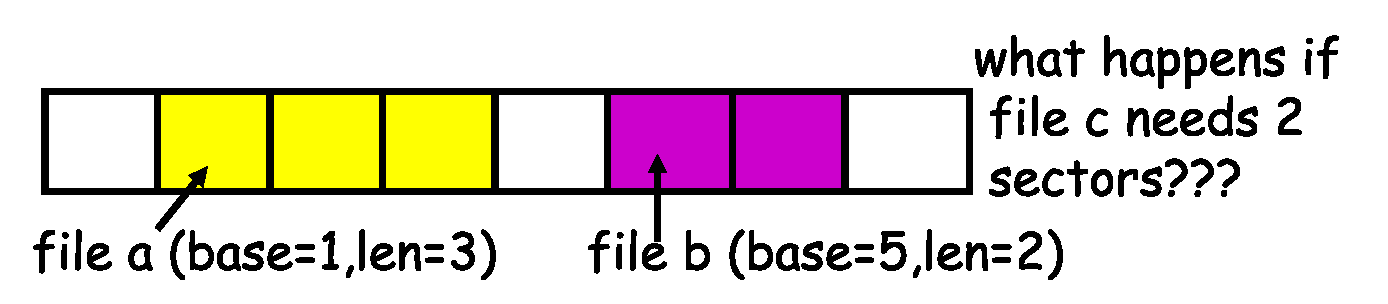
\includegraphics[width=4in]{figs/contig}
  }
  \item Example: IBM OS/360
  \item Pros?
  \ittms{
    \item \onslide<2->{
        Simple, fast access, both sequential and random
    }
  }
  \item Cons? (Think of corresponding VM scheme)
  \ittms{
      \onslide<2->{
        \item External fragmentation
      }
  }
}
\end{slide}

\begin{slide}{Linked files}
\vspace{-1em}
\itms{
  \item Basically a linked list on disk.
  \ittms{
    \item Keep a linked list of all free blocks
    \item Inode contents: a pointer to file's first block
    \item In each block, keep a pointer to the next one \\
\centerline{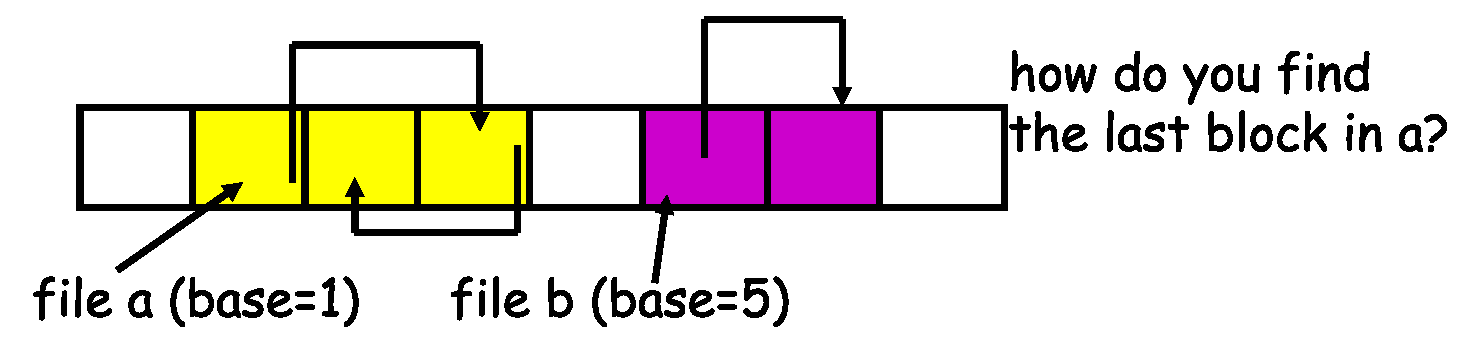
\includegraphics[width=4in]{figs/linked}}
  }
  \item Examples (sort-of): Alto, TOPS-10, DOS FAT
  \item Pros? 
  \ittms{
\onslide<2->{
    \item Easy dynamic growth \& sequential access, no fragmentation
}
  }
  \item Cons? 
  \ittms{
\onslide<2->{
    \item Linked lists on disk a bad idea because of access times
    \item Pointers take up room in block, skewing alignment
}
  }
}
\end{slide}

\begin{frame}
\frametitle{Example: DOS FS (simplified)}
\itms{
  \item Uses linked files.  Cute: links reside in fixed-sized ``file
    allocation table'' (FAT) rather than in the blocks.   \\
%\includegraphics[width=4in]{figs/dos}
\hspace*{1em}%
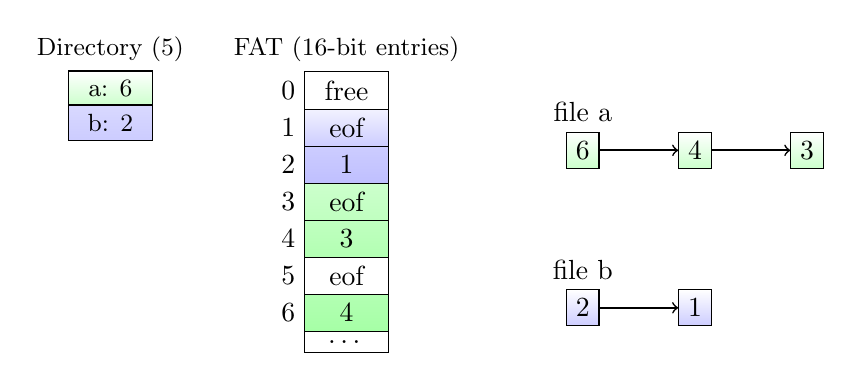
\begin{tikzpicture}[box/.style={draw,minimum width=7ex,on chain,outer
            sep=0pt},
        every join/.style={semithick,->},font=\normalfont,
        ds/.style={drop shadow={shadow xshift=.3ex, shadow yshift=-.3ex}},
    filea/.style={draw=black,shade,top color=white, bottom
        color=green!20},
    fileb/.style={draw=black,shade,top color=white, bottom
        color=blue!20}
    ]
\path[start chain=going below,node
    distance=-.2pt,font=\normalfont\small]
  node[anchor=south,on chain] { Directory (5) }
  node[box,filea]{a: 6}
  node[below,box,fileb,top color=blue!15]{b: 2};
\path[start chain=going below,node distance=0pt] (3,0)
    node[anchor=south,on chain,font=\normalfont\small] { FAT (16-bit entries) }
    node[box,label=left:0] {free}
    node[box,label=left:1,fileb,top color=blue!5] {eof}
    node[box,label=left:2,fileb,top color=blue!20,bottom color=blue!25] {1}
    node[box,label=left:3,filea,top color=green!20,bottom
        color=green!25] {eof}
    node[box,label=left:4,filea,top color=green!25,bottom
        color=green!30] {3}
    node[box,label=left:5] {eof}
    node[box,label=left:6,filea,top color=green!30,bottom
        color=green!35] {4}
    node[box] {\ldots};
\path[start chain=going right] (6,-1)
   node[filea,on chain,label={[fill=none]above:{file a}}]{6}
   node[filea,on chain,join]{4}
   node[filea,on chain,join]{3};
\path[start chain=going right,top color=white,bottom color=blue!20] (6,-3)
   node[fileb,on chain,label=above:{file b}]{2}
   node[fileb,on chain,join]{1};
\end{tikzpicture}
  \item Still do pointer chasing, but can cache entire FAT so can be
    cheap compared to disk access
}
\end{frame}

\begin{slide}{FAT discussion}
\itms{
  \item Entry size = 16 bits
  \ittms{
    \item What's the maximum size of the FAT?
      \onslide<2->{\Maroon{65,536 entries}}
    \item Given a 512 byte block, what's the maximum size of FS?
      \onslide<2->{\Maroon{32 MiB}}
    \item One solution: go to bigger blocks.  Pros?  Cons? 
  }
  \item Space overhead of FAT is trivial:
  \ittms{
    \item 2 bytes / 512 byte block = $\sim0.4\%$ (Compare to Unix) 
  }
  \item Reliability: how to protect against errors? 
  \ittms{
    \item Create duplicate copies of FAT on disk
    \item State duplication a very common theme in reliability
  }
  \item Bootstrapping: where is root directory?
  \ittms{
    \item Fixed location on disk:\quad
\lower 1.5ex\rlap{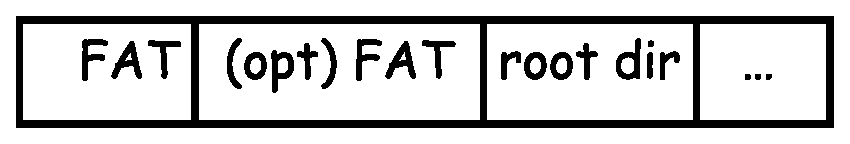
\includegraphics[width=2in]{figs/fatboot}}
  }
}
\end{slide}

\begin{slide}{Indexed files}
\itms{
  \item Each file has an array holding all of it's block pointers
  \ittms{
    \item Just like a page table, so will have similar issues
    \item Max file size fixed by array's size (static or dynamic?)
    \item Allocate array to hold file's block pointers on file
      creation
    \item Allocate actual blocks on demand using free list
  } 
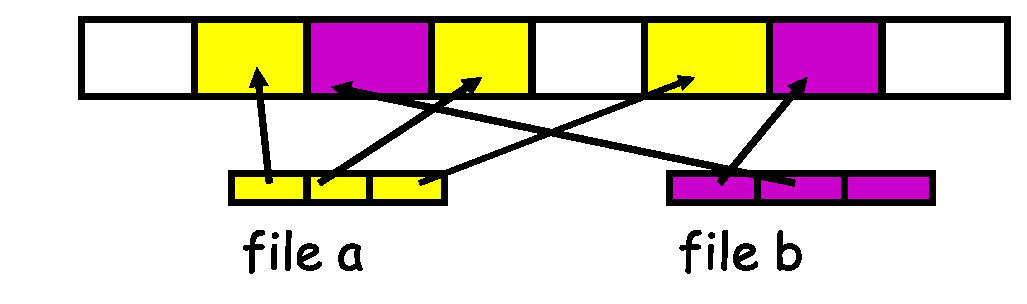
\includegraphics[width=3.5in]{figs/indexed}
\vspace*{-.3in}
  \item Pros?
  \ittms{
\onslide<2->{
    \item Both sequential and random access easy
}
  }
  \item Cons?
  \ittms{
\onslide<2->{
    \item Mapping table requires large chunk of contiguous space \\
        \ldots Same problem we were trying to solve initially
}
  }
}
\end{slide}

\begin{slide}{Indexed files}
\itms{
  \item Issues same as in page tables \\
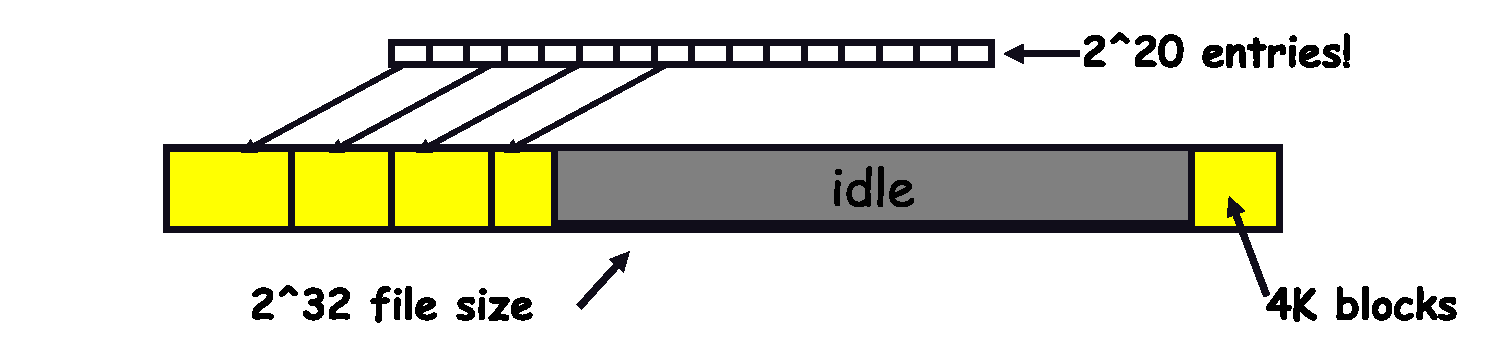
\includegraphics[width=4in]{figs/pagetb}
  \ittms{
    \item Large possible file size = lots of unused entries
    \item Large actual size? table needs large contiguous disk chunk
  }
  \item Solve identically: small regions with index array, this array
    with another array, \ldots  \ Downside? \\
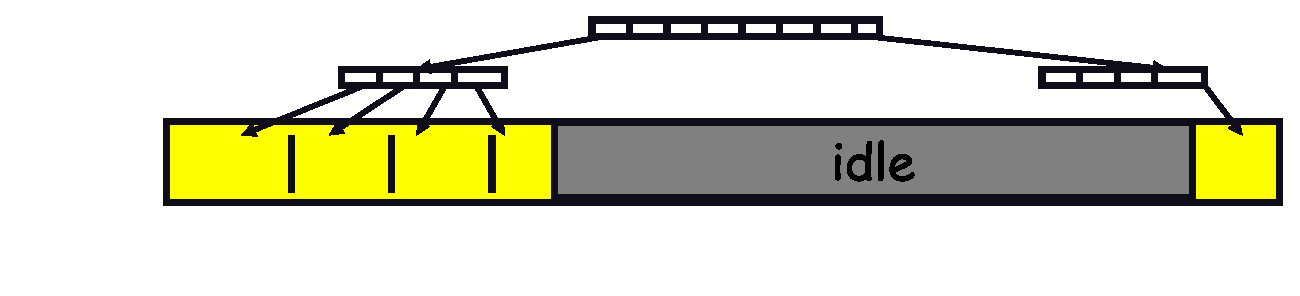
\includegraphics[width=4in]{figs/hpagetb}
}
\end{slide}

\begin{slide}{Multi-level indexed files (old BSD FS)}
\itms{
  \item Solve problem of first block access slow
  \item inode = 14 block pointers + ``stuff''
}
\centerline{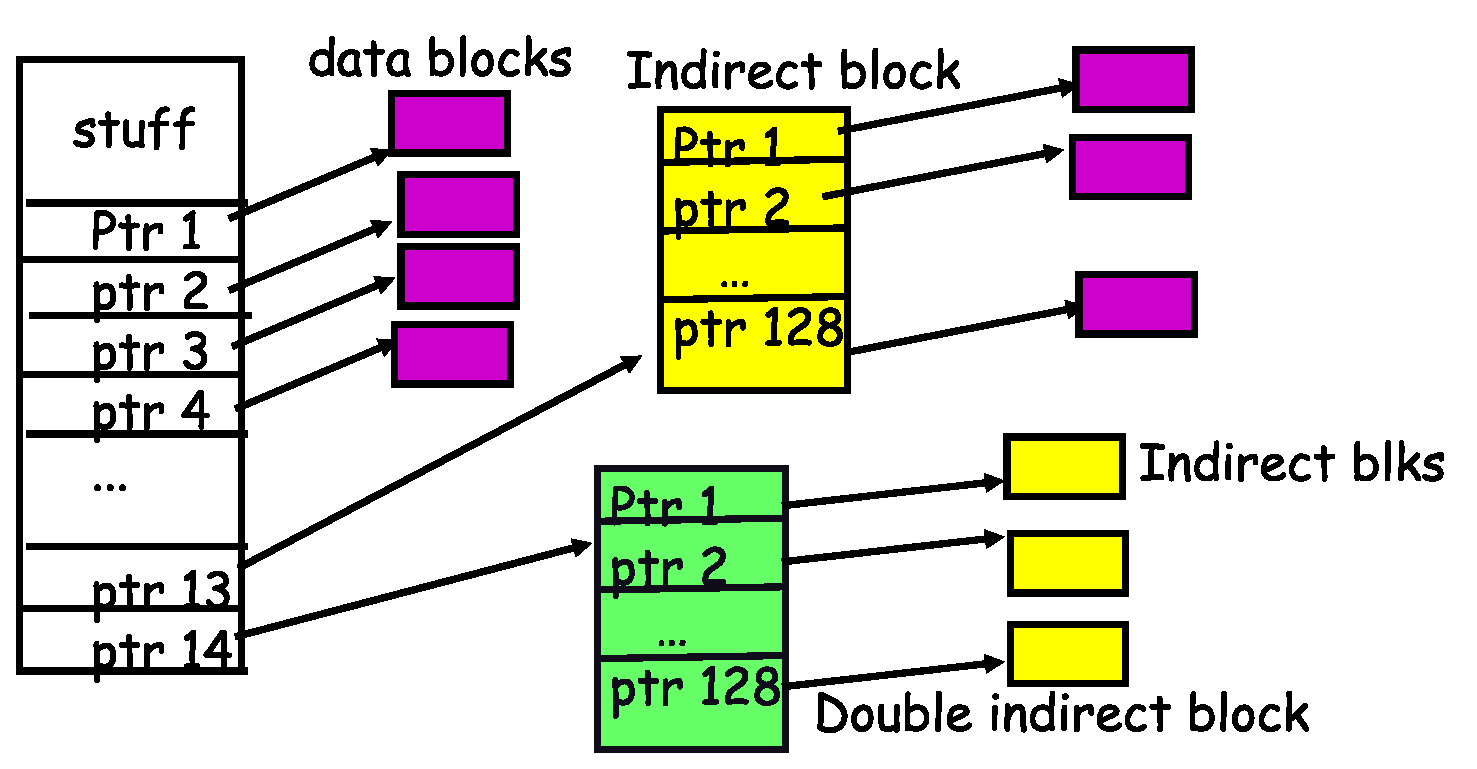
\includegraphics[width=4.8in]{figs/43bsd}}
\end{slide}

\begin{slide}{Old BSD FS discussion}
\itms{
  \item Pros:
  \ittms{
    \item Simple, easy to build, fast access to small files
    \item Maximum file length fixed, but large. %(With 4k blks?)
  }
  \item Cons:
  \ittms{
    \item What is the worst case \# of accesses?
    \item What is the worst-case space overhead? (e.g., 13~block file)
  }
  \item An empirical problem:
  \ittms{
  \item Because you allocate blocks by taking them off unordered
    freelist, metadata and data get strewn across disk
  }
}
\end{slide}

\begin{slide}{More about inodes}
\vspace{-1em}
\itms{
  \item Inodes are stored in a fixed-size array
  \ittms{
  \item Size of array fixed when disk is initialized; can't be changed
  \item Lives in known location, originally at one side of disk: \\
    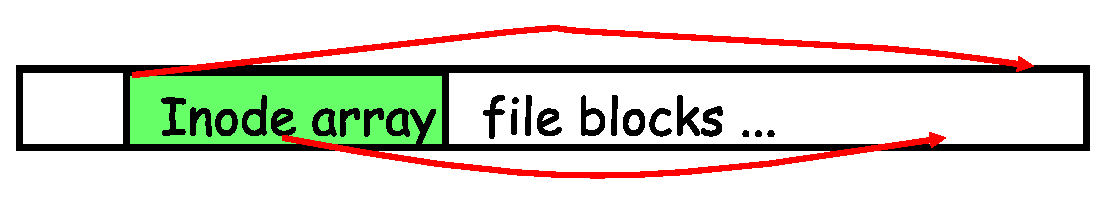
\includegraphics[width=4in]{figs/inode1}
\vspace*{-.1in}
  \item Now is smeared across it (why?) \\
    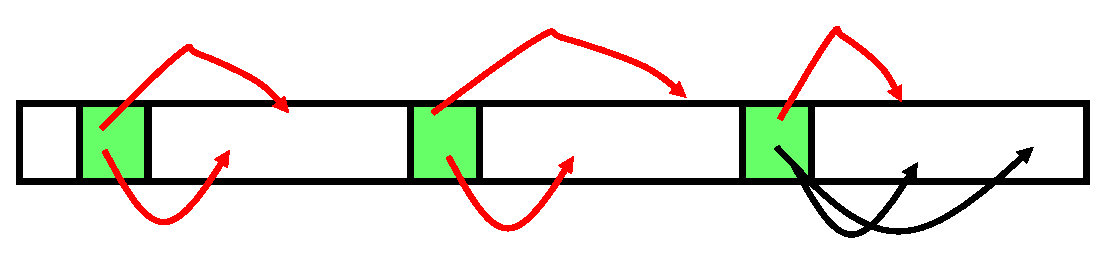
\includegraphics[width=4in]{figs/inode2}
\vspace*{-.1in}
    \item The index of an inode in the inode array called an i-number
    \item Internally, the OS refers to files by inumber
    \item When file is opened, inode brought in memory
    \item Written back when modified and file closed or time elapses
  }
}
\end{slide}

%% \begin{slide}{Example: (oversimplified) Unix FS}
%% \itms{
%%   \item Want to modify byte 4 in \texttt{/a/b.c}:
%% }
%% \vbox to 1.1in{
%% \kern-.1in
%% \centerline{\hspace*{.4in}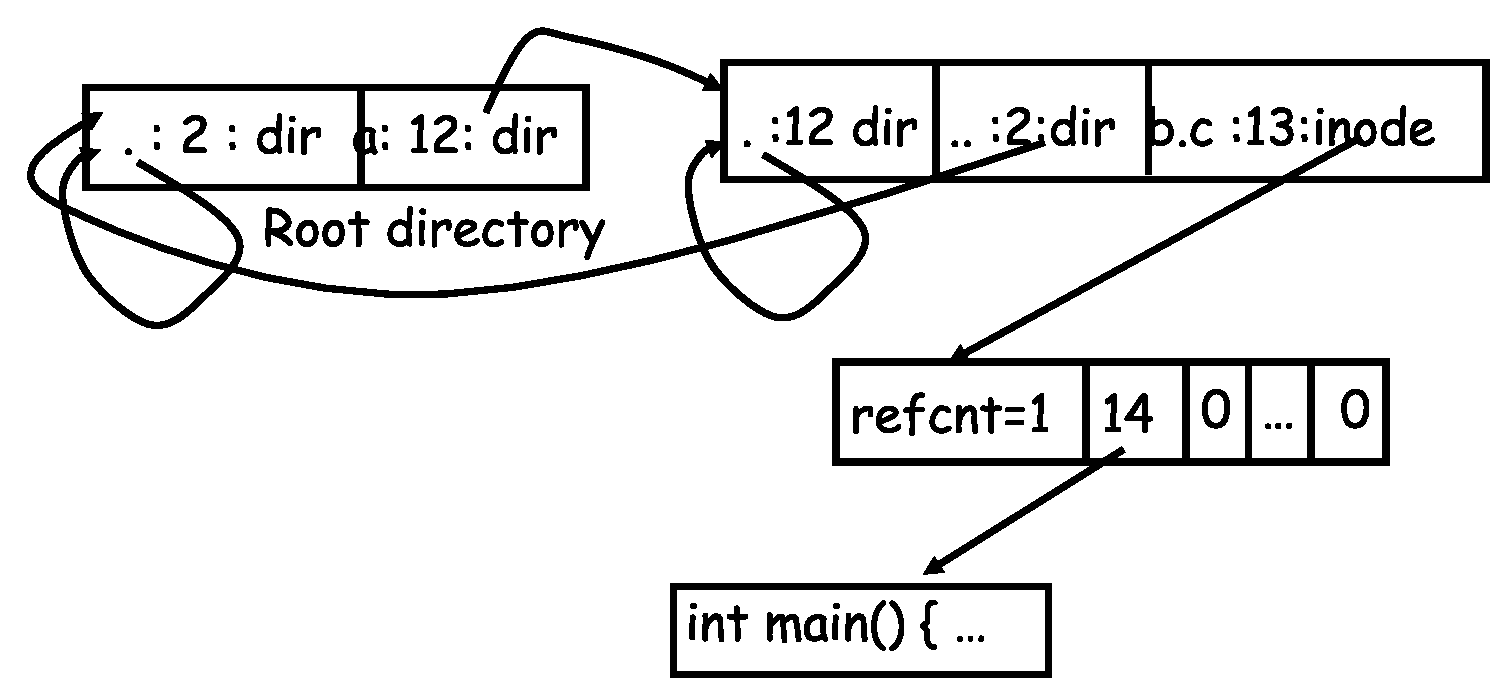
\includegraphics[width=4in]{figs/unix}}
%% \hbox{}
%% \vss
%% }
%% \hspace*{-.2in}\begin{minipage}{4in}
%%   \ittms{
%%     \item readin root directory (inode 2)
%%     \item lookup a (inode 12); readin
%%     \item lookup inode for b.c (13); readin
%%     \item use inode to find blk for byte 4 (blksize = 512, so offset = 0 gives blk 14); readin and modify
%%   }
%% \end{minipage}
%% \end{slide}

\begin{slide}{Directories}
\itms{
  \item Problem: 
  \ittms{
  \item ``Spend all day generating data, come back the next morning,
    want to use it.'' -- F. Corbato, on why files/dirs invented
  }
  \item Approach 0: Have users remember where on disk their files are
  \ittms{
    \item (E.g., like remembering your social security or bank account \#)
  }
  \item Yuck.  People want human digestible names
  \ittms{
    \item We use directories to map names to file blocks 
  }
  \item Next: What is in a directory and why?
}
\end{slide}

\begin{slide}{A short history of directories}
\vspace*{-.1in}
\itms{
  \item Approach 1: Single directory for entire system
  \ittms{
    \item Put directory at known location on disk
    \item Directory contains $\langle\mathrm{name, inumber}\rangle$ pairs
    \item If one user uses a name, no one else can
    \item Many ancient personal computers work this way % (cf ``hosts.txt'')
  }
  \item Approach 2: Single directory for each user
  \ittms{
    \item Still clumsy, and \texttt{ls} on 10,000 files is a real pain
    %\item (many older mathematicians work this way)
  }
  \item Approach 3: Hierarchical name spaces
  \ittms{
    \item Allow directory to map names to files \emph{or other dirs}
    \item File system forms a tree (or graph, if links allowed)
    \item Large name spaces tend to be hierarchical (ip addresses, domain names, scoping in programming languages, etc.)
  }
}
\end{slide}

\begin{frame}
\frametitle{Hierarchical Unix}
\itms{
  \item Used since CTSS (1960s)
\vadjust{\moveright 2.8in\vbox to.0pt{\vss
    \hbox{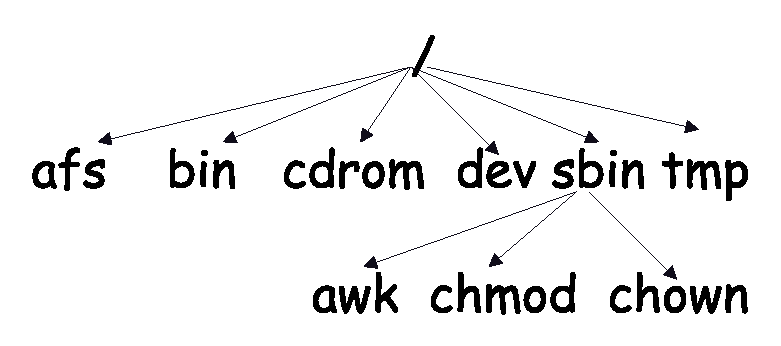
\includegraphics[width=2in]{figs/tree}}\kern-.5in\hbox{}}}
  \ittms{
    \item Unix picked up and used really nicely
  }
  \item Directories stored on disk just like regular files \\[-1ex]
\begin{columns}[T]
\column{.6\textwidth}
  \ittms{
    \item Special inode type byte set to directory
    \item User's can read just like any other file
    \item Only special syscalls can write (why?)
    \item Inodes at fixed disk location
    \item File pointed to by the index may be \\
      another directory
    \item Makes FS into hierarchical tree						(what needed to make a DAG?)
  }
\column{.3\textwidth}
\vspace*{1em}
{\color[rgb]{.5,0,1}\tt
\begin{tabular}{|r@{,}l|}
\hline
<\normalfont\itshape name&{\normalfont\itshape inode}\#>\cr
<afs&1021>\cr
<tmp&1020>\cr
<bin&1022>\cr
<cdrom&4123>\cr
<dev&1001>\cr
<sbin&1011>\cr
\omit\vrule&\omit$\vdots$\vrule width 0pt depth 3pt \hfil\vrule\cr
\hline
\end{tabular}
}
\end{columns}
  \item Simple, plus speeding up file ops speeds up dir ops! 
}
\end{frame}

\begin{slide}{Naming magic}
\itms{
  \item Bootstrapping: Where do you start looking?  
  \ittms{
    \item Root directory always inode \#2 (0 and 1 historically
      reserved)
  }
  \item Special names:
  \ittms{
    \item Root directory: ``\texttt{/}''	
    \item Current directory: ``\texttt{.}''
    \item Parent directory: ``\texttt{..}'' 
  }
  \item Special names not implemented in FS:
  \ittms{
    \item User's home directory: ``$\sim$''
    \item Globbing: ``\texttt{foo.*}'' expands to all files starting
      ``\texttt{foo.}''
  }
  \item Using the given names, only need two operations to navigate the entire name space:
  \ittms{
    \item \texttt{cd} \emph{name}: move into (change context to)
      directory \emph{name}
    \item \texttt{ls}: enumerate all names in current directory (context)
  }
}
\end{slide}

\begin{slide}{Unix example: \texttt{/a/b/c.c}}
\centerline{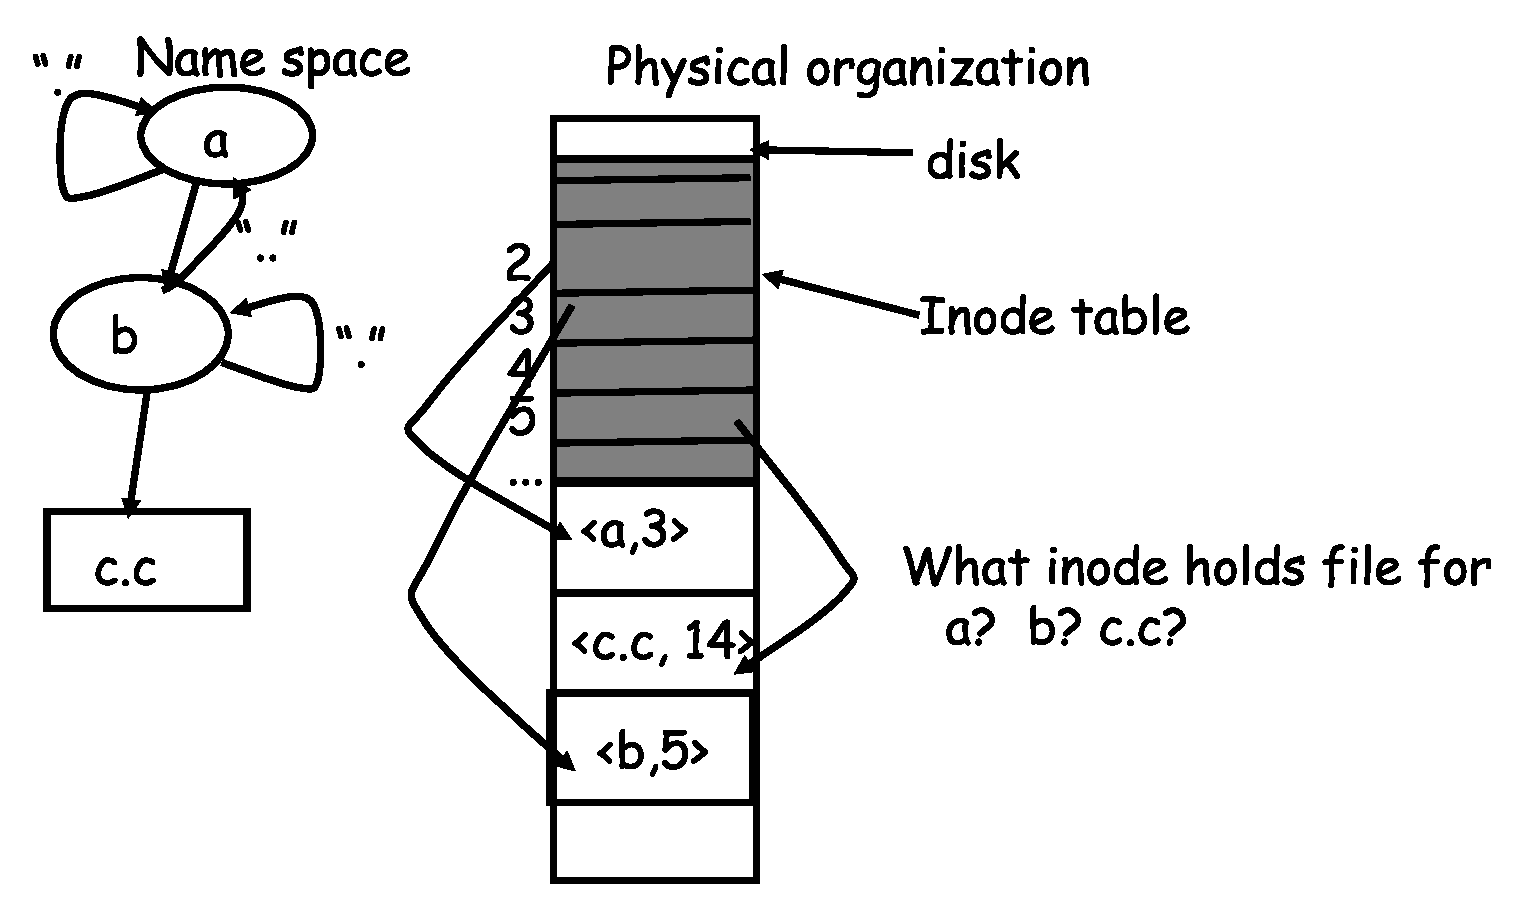
\includegraphics[width=4.9in]{figs/unix-example}}
\end{slide}

\begin{slide}{Default context: working directory}
\itms{
  \item Cumbersome to constantly specify full path names
  \ittms{
    \item In Unix, each process associated with a ``current working
      directory'' (cwd)
    \item File names not beginning with ``/'' are assumed to be
      relative to cwd; otherwise translation happens as before
    \item Editorial: root, cwd should be regular fds (like stdin,
      stdout,~\ldots) with \emph{openat} syscall instead of
      \emph{open}
  }
  \item Shells track a default list of active contexts 
  \ittms{
    \item A ``search path'' for programs you run
    \item Given a search path $A:B:C$, a shell will check in A, then check in B, then check in C
    \item Can escape using explicit paths: ``./foo''
  }
  \item Example of locality
}
\end{slide}

\begin{frame}
\frametitle{Hard and soft links (synonyms)}
\itms{
  \item More than one dir entry can refer to a given file
\vspace*{-1ex}
    \begin{columns}[T]
        \column{60mm}
      \ittms{
        \item Unix stores count of pointers (``hard links'') to inode
        \item To make: ``\texttt{ln foo bar}'' creates a synonym
          (\texttt{bar}) for \emph{file} \texttt{foo}
      }
        \column{30mm}
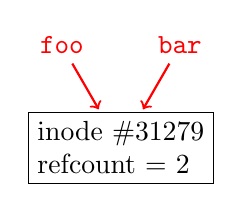
\begin{tikzpicture}[font=\normalfont,remember picture]
\path node[draw,align=left] (inode) {inode \#31279\\ refcount = 2}
  node[red,font=\ttfamily] at (120:1.5) {foo}
    edge[red,thick,->,shorten >=1pt] (inode)
  node[red,font=\ttfamily] at (60:1.5) (bar) {bar}
    edge[red,thick,->,shorten >=1pt] (inode) ;
\end{tikzpicture}
    \end{columns}
  \item Soft/symbolic links = synonyms for \emph{names}
  \ittms{
    \item Point to a file (or dir) \emph{name}, but object can be
      deleted from underneath it (or never even exist).
    \item Unix implements like directories: inode has special \\
      ``symlink'' bit set and contains name of link target \\
      \leavevmode\raise 2.5ex\hbox{\quad\texttt{ln -s /bar baz} }
\begin{tikzpicture}[remember picture,font=\normalfont\normalsize]
\path node[draw,align=left] (symlink) {\texttt{"/bar"}\\ refcount = 1}
  edge[->,dotted,red,thick,overlay,out=0,in=-10,looseness=1.1] (bar)
  node[red,font=\ttfamily\normalsize] at (-170:2.2) {baz}
    edge[red,thick,->,shorten >=1pt] (symlink);
\end{tikzpicture}
    \item When the file system encounters a symbolic link it
      automatically translates it (if possible).
  }
}
\end{frame}

\begin{slide}{Case study: speeding up FS}
\itms{
  \item Original Unix FS: Simple and elegant: \\
    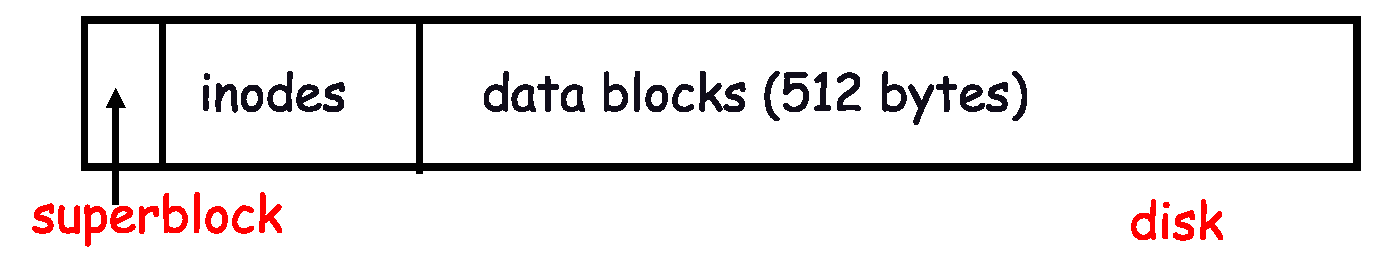
\includegraphics[width=4in]{figs/origunix}
  \item Components: 
  \ittms{
    \item Data blocks 
    \item Inodes (directories represented as files)
    \item Hard links
    \item Superblock. (specifies number of blks in FS, counts of max
      \# of files, pointer to head of free list)
  }
  \item Problem: slow
  \ittms{
    \item Only gets 20Kb/sec (2\% of disk maximum) even for sequential disk transfers!
  }
}
\end{slide}

\begin{slide}{A plethora of performance costs}
\itms{
  \item Blocks too small (512 bytes)
  \ittms{
    \item File index too large 
    \item Too many layers of mapping indirection
    \item Transfer rate low (get one block at time)
  }

  \item Poor clustering of related objects:
  \ittms{
    \item Consecutive file blocks not close together
    \item Inodes far from data blocks
    \item Inodes for directory not close together
    \item Poor enumeration performance:  e.g., ``\texttt{ls}'',
      ``\texttt{grep foo *.c}''
  }
  \item Usability problems
  \begin{itemize}
    \item 14-character file names a pain
    \item Can't atomically update file in crash-proof way
  \end{itemize}
  \item Next: how FFS fixes these (to a degree)
    \cref{sched/readings/ffs.pdf}{[McKusic]}
}
\end{slide}

\begin{slide}{Problem:  Internal fragmentation}
\itms{
  \item Block size was too small in Unix FS
  \item Why not just make block size bigger? \\[1ex]
\hspace*{1em}\Blue{
\begin{tabular}{|l|l|l|}
\hline
Block size & space wasted & file bandwidth \\
512        &    6.9\%     &             2.6\% \\
1024       &    11.8\%    &             3.3\% \\
2048       &    22.4\%    &             6.4\% \\
4096       &    45.6\%    &             12.0\% \\
1MB        &    99.0\%    &             97.2\% \\
\hline
    \end{tabular}
}
\bigskip

  \item Bigger block increases bandwidth, but how to deal with wastage (``internal fragmentation'')?
  \ittms{
    \item Use idea from malloc: split unused portion.
  }
}
\end{slide}

\begin{slide}{Solution: fragments}
\itms{
  \item BSD FFS: 
  \ittms{
    \item Has large block size (4096 or 8192)
    \item Allow large blocks to be chopped into small ones (``fragments'')
    \item Used for little files and pieces at the ends of files \\
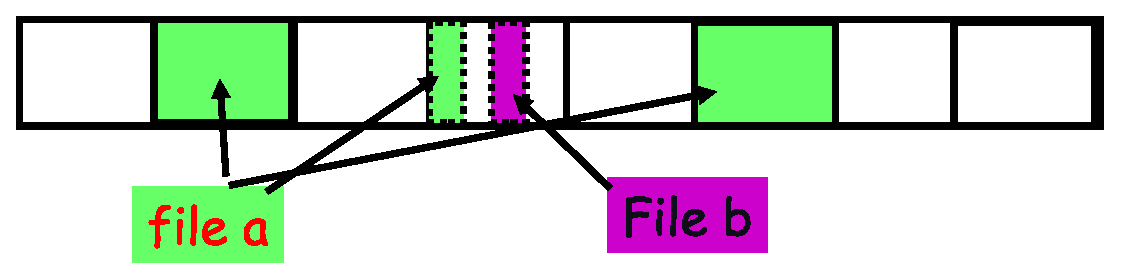
\includegraphics[width=4in]{figs/fragments}      
  }
  \item Best way to eliminate internal fragmentation?
  \ittms{
    \item Variable sized splits of course
    \item Why does FFS use fixed-sized fragments (1024, 2048)?
  }
}
\end{slide}

\begin{slide}{Clustering related objects in FFS}
\itms{
  \item Group 1 or more consecutive cylinders into a ``\Red{\emph{cylinder
    group}}'' \\
  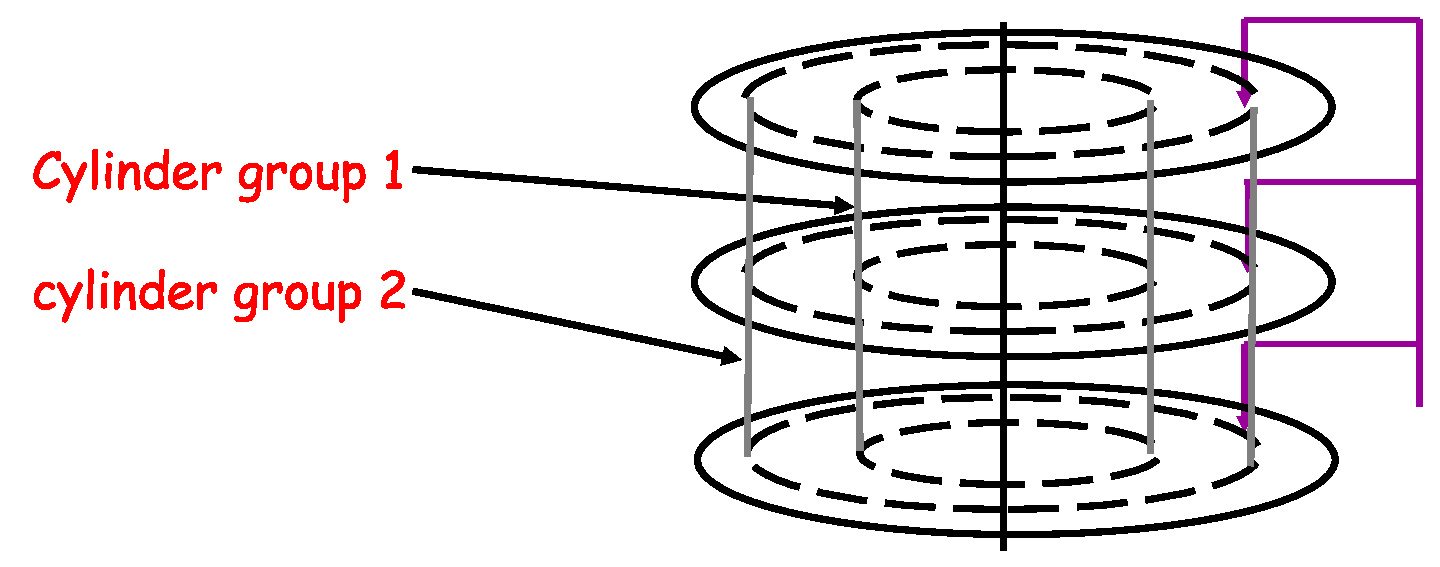
\includegraphics[width=4in]{figs/cgroup}
  \ittms{
    \item Key: can access any block in a cylinder without performing a seek.  Next fastest place is adjacent cylinder.
    \item Tries to put everything related in same cylinder group
    \item Tries to put everything not related in different group (?!)
  }
}
\end{slide}

\begin{slide}{Clustering in FFS}
\itms{
  \item Tries to put sequential blocks in adjacent sectors
  \ittms{
    \item (Access one block, probably access next) \\
      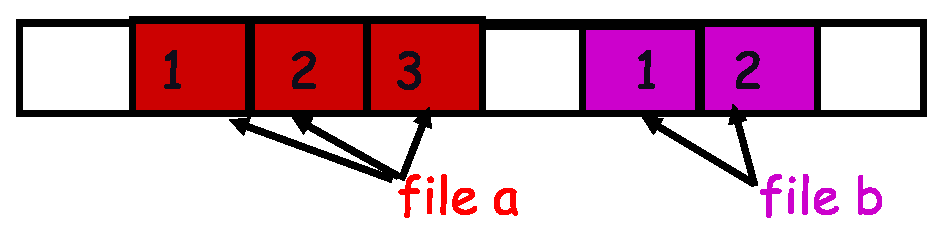
\includegraphics[width=3.2in]{figs/cg1}
  }
  \item Tries to keep inode in same cylinder as file data:
  \ittms{
    \item (If you look at inode, most likely will look at data too) \\
      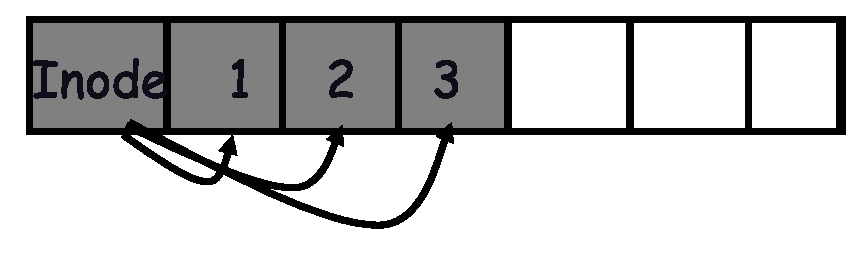
\includegraphics[width=3.2in]{figs/cg2}
  }
  \item Tries to keep all inodes in a dir in same \rlap{cylinder
    group}
  \ittms{
    \item Access one name, frequently access many, e.g., ``\texttt{ls
        -l}''   
  }
}
\end{slide}

\begin{slide}{What does disk layout look like?}
\itms{
  \item Each cylinder group basically a mini-Unix file system: \\
    \hspace*{1em}\input{ffs}
    %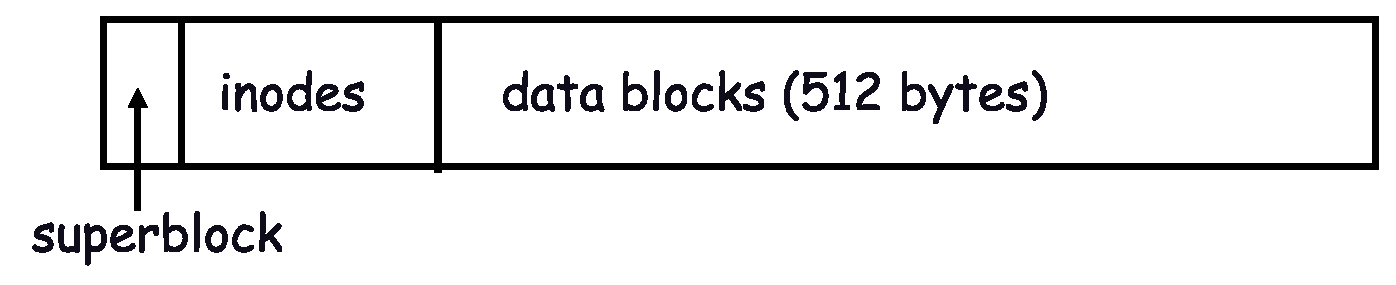
\includegraphics[width=4in]{figs/cg3}
  \item How how to ensure there's space for related stuff?
  \ittms{
    \item Place different directories in different cylinder groups
    \item Keep a ``free space reserve'' so can allocate near existing things
    \item When file grows too big (1MB) send its remainder to
      different cylinder group.
  }
}
\end{slide}

\begin{slide}{Finding space for related objs}
\itms{
  \item Old Unix (\& DOS): Linked list of free blocks
  \ittms{
    \item Just take a block off of the head.  Easy. 
      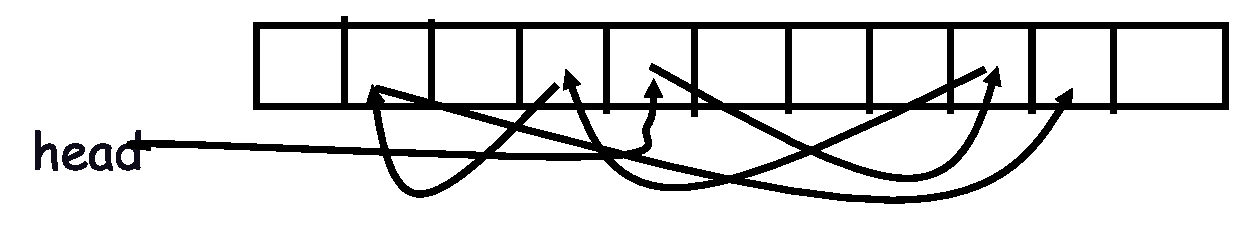
\includegraphics[width=4in]{figs/linkedlist}
    \item Bad: free list gets jumbled over time.  Finding adjacent blocks hard and slow 
  }
  \item FFS: switch to bit-map of free blocks
  \ittms{
    \item 1010101111111000001111111000101100
    \item Easier to find contiguous blocks.  
    \item Small, so usually keep entire thing in memory
    \item Time to find free block increases if fewer free blocks
%    \item If very few free blocks, will be slow to find one.\\
%      Solution: Keep a reserve of free blocks (e.g., 5\%)
  }
}
\end{slide}

\begin{slide}{Using a bitmap}
\itms{
  \item Usually keep entire bitmap in memory:
  \ittms{
    \item 4G disk / 4K byte blocks.  How big is map?
  }
  \item Allocate block close to block $x$?
  \ittms{
    \item Check for blocks near \texttt{bmap[$x$/32]}
    \item If disk almost empty, will likely find one near
    \item As disk becomes full, search becomes more expensive and less
      effective
  }
  \item Trade space for time (search time, file access time)
  \item Keep a reserve (e.g, 10\%) of disk always free, ideally scattered across disk
  \ittms{
    \item Don't tell users (\texttt{df} can get to 110\% full)
    \item Only root can allocate blocks once FS 100\% full
    %\item $N$ platters = $N$ adjacent blocks
    \item With 10\% free, can almost always find one of them free
  }
}
\end{slide}

\begin{slide}{So what did we gain?}
\itms{
  \item Performance improvements:
  \ittms{
    \item Able to get 20-40\% of disk bandwidth for large files
    \item 10-20x original Unix file system!
    \item Better small file performance  (why?)
  }
  \item Is this the best we can do?  No.
  \item Block based rather than extent based
  \ittms{
    \item Could have named contiguous blocks with single pointer and length
    (Linux ext2fs, XFS)
  }
  \item Writes of metadata done synchronously
  \ittms{
    \item Really hurts small file performance
    \item Make asynchronous with write-ordering (``soft updates'') or
      logging/journaling\ldots\ more next lecture
      %(the episode file system, $\sim$LFS)
    \item Play with semantics (/tmp file systems)
  }
}
\end{slide}

\begin{slide}{Other hacks}
\itms{
  \item Obvious:
  \ittms{
    \item Big file cache
  }
  \item Fact: no rotation delay if get whole track.
  \ittms{
    \item How to use?
  }
  \item Fact: transfer cost negligible.
  \ittms{
    \item Recall:  Can get 50x the data for only $\sim$3\% more overhead
    \item 1 sector: 5ms + 4ms + 5$\mu$s
      $\left(\mathrm{\approx 512\>B/(100\>MB/s)}\right)$ $\approx$ 9ms
    \item 50 sectors: 5ms + 4ms + .25ms = 9.25ms
    \item How to use?
  }
  \item Fact: if transfer huge, seek + rotation negligible
  \ittms{
    \item \href{http://www.stanford.edu/~ouster/cgi-bin/papers/lfs.pdf}{LFS}:
      Hoard data, write out MB at a time
  }
}
\end{slide}

\end{document}
